We use MCFM v6.0 NLO generator to extract the leading lepton pt
distribution for SM and aTGC points, which are used to derive final
results. We also use the Sherpa event generator with the standard
FastSim sequence to produce samples of approximately 20,000 \ww\
events with and without anomalous couplings.  The leading lepton
distribution is found to be consistent between the two approaches as
one can see in Figure~\ref{fig:generator_comparison}.
\begin{figure}[tp]
  \centerline{
    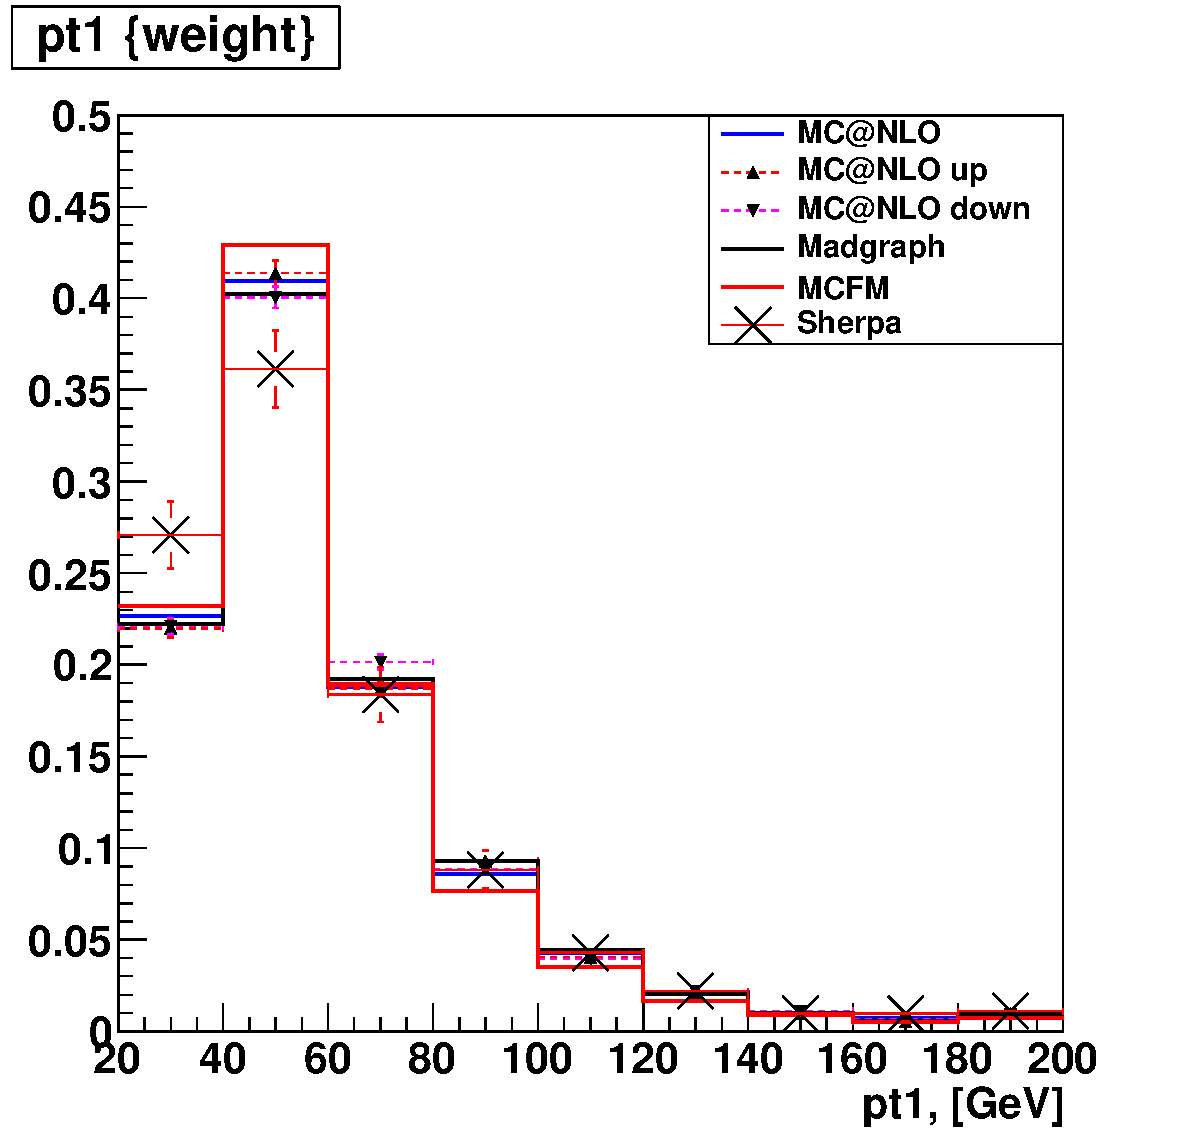
\includegraphics[width=0.6\textwidth]{figures/generator_comparison.pdf}
%    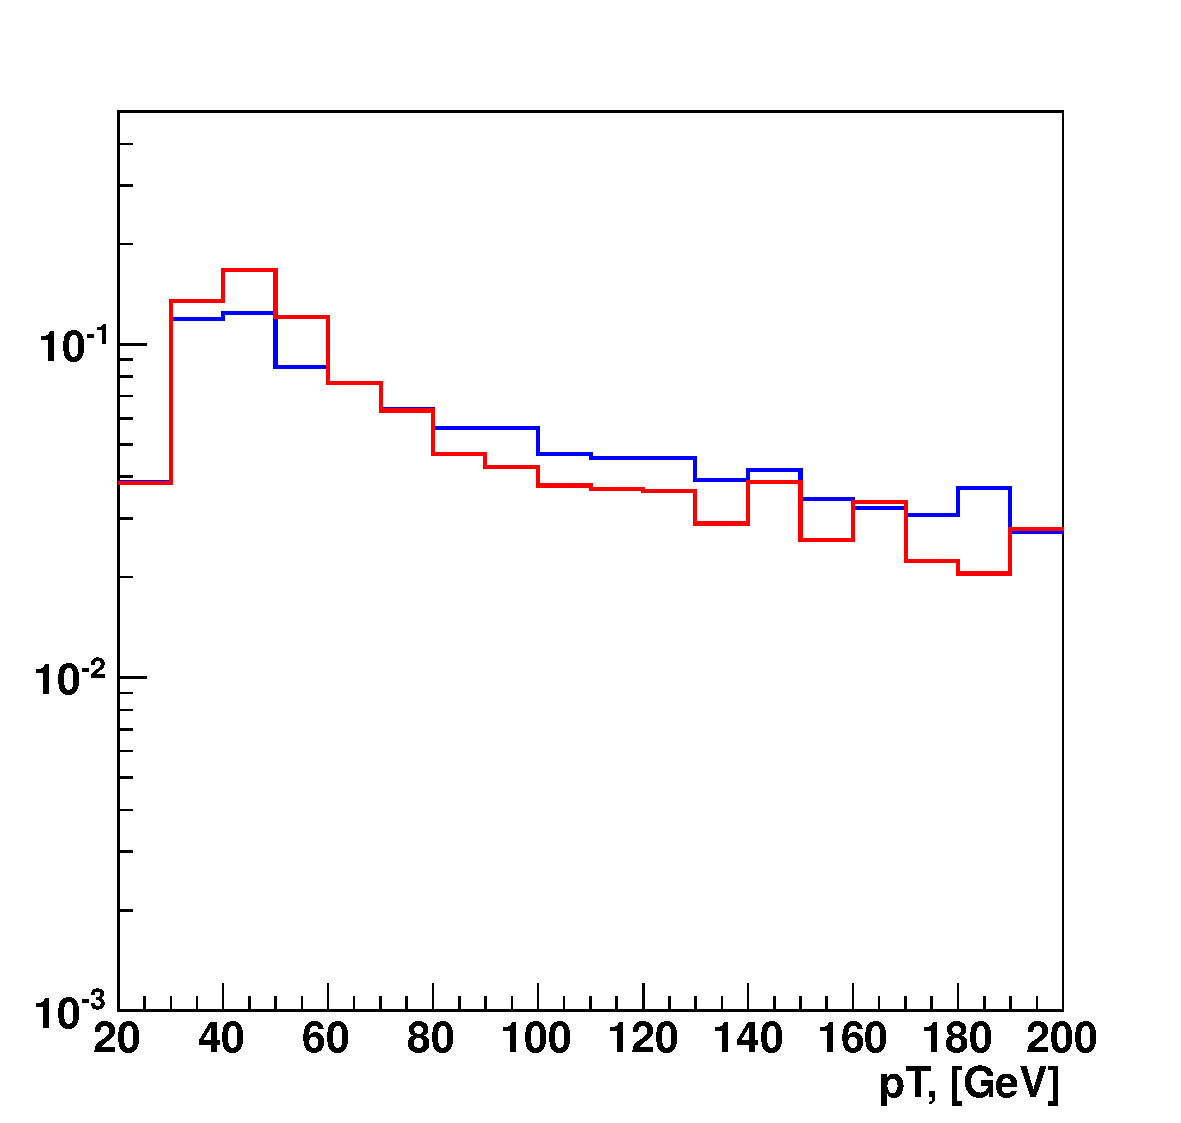
\includegraphics[width=0.45\textwidth]{figures/generator_comparison_atgc.pdf}
  }

  \caption[Generator comparison]{Leading lepton \pt\ distribution
  for \WW\ simulated data using Madgraph (full simulation), MC@NLO (full simulation),
  Sherpa (fast simulation) and MCFM (reweighted). No aTGC.}

  \label{fig:generator_comparison}
\end{figure}

The anomalous coupling samples were produced with couplings listed in
Table~\ref{tab:xsections} in which one is the Standard Model value,
and the other two coupling values vary.
